% !TEX root = main.tex
% --+ 11.51 INTRODUCTION +------------------------------------------------------
\begin{frame}{Acceptance Correction: Generation + Simulation}
    \label{11.51::introduction}
    \begin{itemize}
        \item
            To apply acceptance correction, 10M DIS events were generated in \ef{LEPTO}.

        \item
            Then, they were simulated with \ef{GEMC 5.2} with run 12016's conditions.

        \item
            Finally, they were reconstructed with \ef{Coatjava 8.2.0}.
    \end{itemize}

    \vspace{-12pt}

    \begin{columns}[onlytextwidth,T]

    \begin{column}{.05\linewidth}\end{column} % Centering column.

    \begin{column}{.35\linewidth}
        \begin{center}
            \begin{figure}[t]
                \centering{
                    \fbox{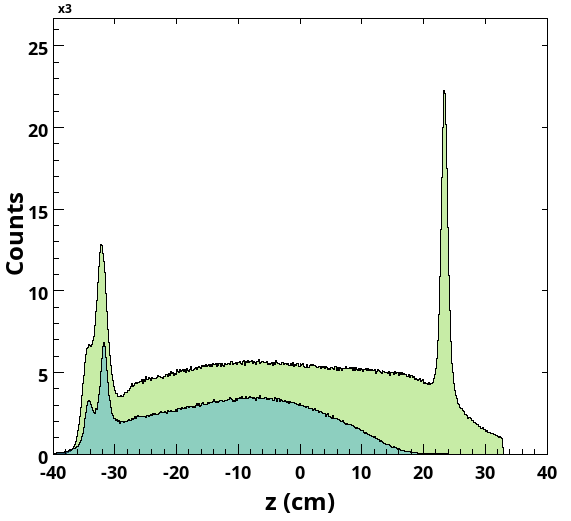
\includegraphics[width=\textwidth]{51vz_012016.png}}
                }
                \textit{Run \ef{12016}.}
            \end{figure}
        \end{center}
    \end{column}

    \begin{column}{.35\linewidth}
        \begin{center}
            \begin{figure}[t]
                \centering{
                    \fbox{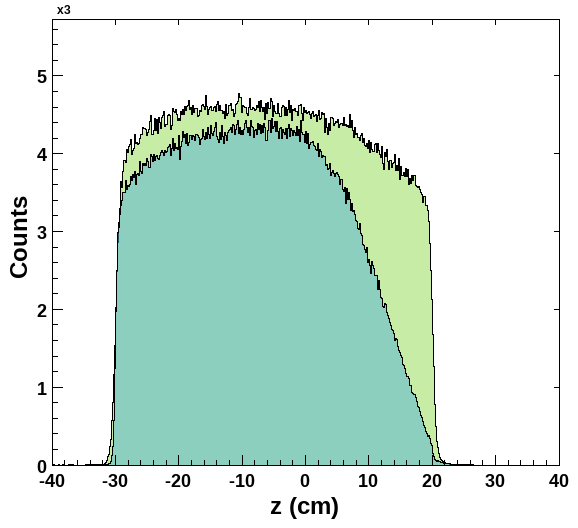
\includegraphics[width=\textwidth]{51vz_999106.png}}
                }
                \textit{Simulated data.}
            \end{figure}
        \end{center}
    \end{column}

    \begin{column}{.05\linewidth}\end{column} % Centering column.

    \end{columns}

    \begin{center}
        \textit{\ef{$v_z$} for \textbf{\textcolor[HTML]{c7eca6}{DC (green)}} and \textbf{\textcolor[HTML]{8dcfbf}{FMT (cyan)}} tracks}
    \end{center}
\end{frame}

% --+ 11.52 ELECTRON VARIABLES +------------------------------------------------
\begin{frame}{Acceptance Correction: $Q^2$}
    \label{11.52::electron_variables}

    \begin{itemize}
        \item
            A drop in \ef{$Q^2$} acceptance is perceived from \ef{1 to 4 $\text{GeV}^2$}.

        \item
            \ef{$\nu$} is within expected parameters.
    \end{itemize}

    \vspace{-12pt}
    \begin{columns}[onlytextwidth,T]

    \begin{column}{.49\linewidth}
        \begin{center}
            \begin{figure}[t]
                \centering{
                    \fbox{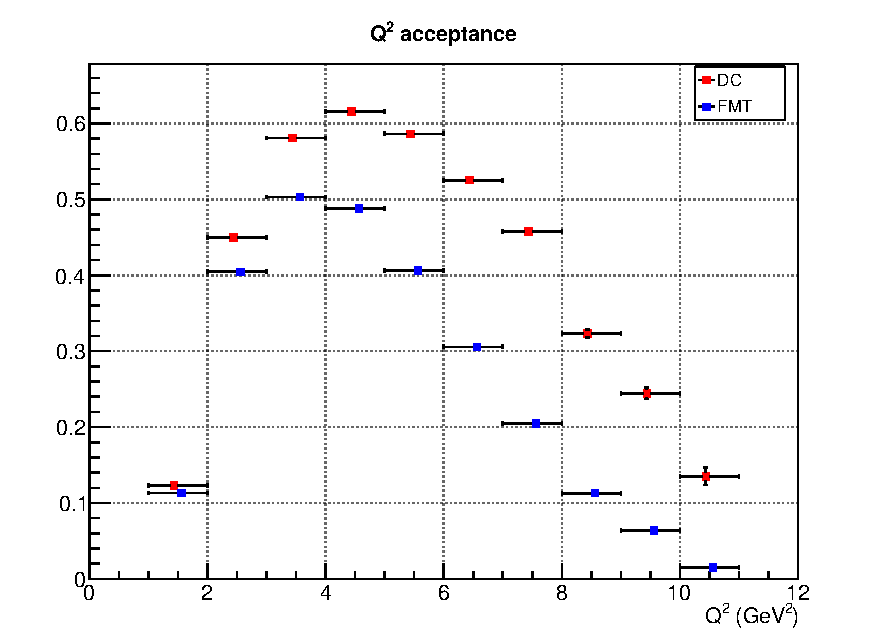
\includegraphics[width=\textwidth]{52q2_acc.pdf}}
                }
                \textit{\ef{$Q^2$} acceptance for \ef{$e^-$}.}
            \end{figure}
        \end{center}
    \end{column}

    \begin{column}{.49\linewidth}
        \begin{center}
            \begin{figure}[t]
                \centering{
                    \fbox{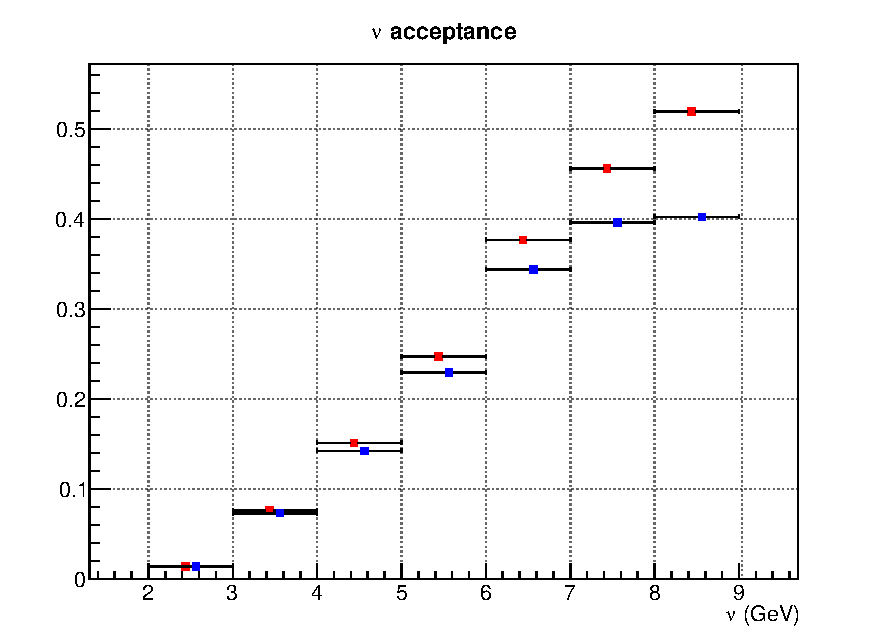
\includegraphics[width=\textwidth]{52nu_acc.pdf}}
                }
                \textit{\ef{$\nu$} acceptance for \ef{$e^-$}.}
            \end{figure}
        \end{center}
    \end{column}

    \end{columns}

    \begin{flushright}
        \tiny{\textit{Bin markers are slightly shifted in $x$ for legibility.}}
        \tiny{\textit{Acceptance error estimation is shown in Slides \textcolor{efd_purple}{\ref{20.05::acceptance_error_estimation}} to \textcolor{efd_purple}{\ref{20.05::acceptance_error_estimation_end}}.}}
    \end{flushright}
\end{frame}

% --+ 11.53 Q2 THETA DEPENDENCE +-----------------------------------------------
\begin{frame}{Acceptance Correction: $Q^2$ $\theta$ dependence}
    \label{11.53::q2_theta_dependence}

    \begin{itemize}
        \item
            \ef{$Q^2$} depends quadratically on the scattered \ef{$e^-$} scattering angle \ef{$\theta_C$}.

        \item
            The CLAS12 Forward Detector has a small efficiency for \ef{$\theta \lsim 0.15$} radians.

        \item
            This causes the drop in acceptance - \ef{it is a purely geometric effect}.
    \end{itemize}

    \begin{center}
        \begin{figure}[t]
            \centering{
                \fbox{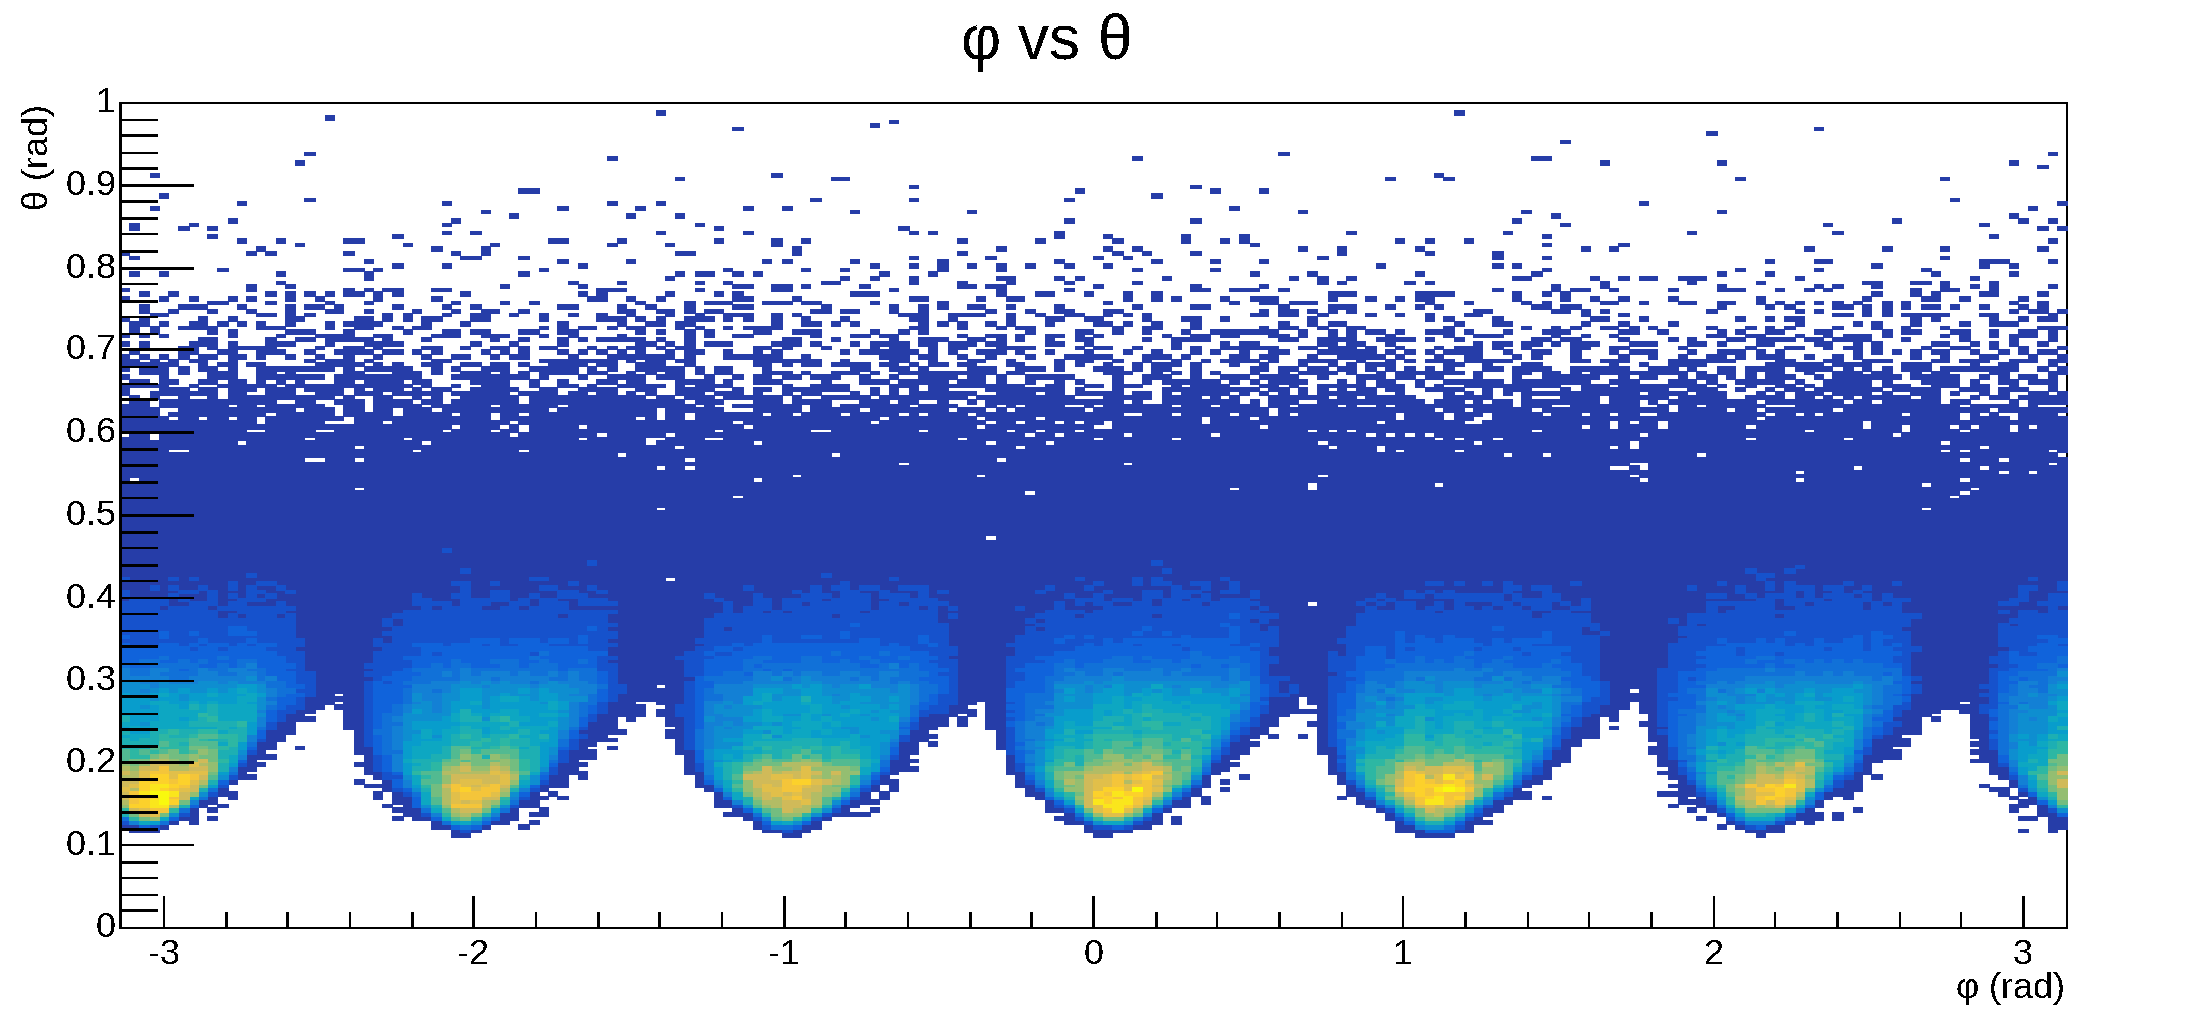
\includegraphics[width=0.8\textwidth]{53phi_theta_neg.pdf}}
            }
        \end{figure}
        \textit{\ef{$\varphi$} vs \ef{$\theta$} for negative particles}
    \end{center}
\end{frame}

% --+ THE REST +----------------------------------------------------------------
% \begin{frame}{Acceptance Correction: $z_h$}
%     \vspace{-18pt}
%     \begin{columns}
%         \begin{column}{.05\linewidth}\end{column} % Centering column.

%         \begin{column}{.40\linewidth}
%             \begin{center}
%                 \begin{figure}[t]
%                     \centering{
%                         \fbox{\includegraphics[width=\textwidth]{zh_acc_211.pdf}}
%                     }
%                 \end{figure}
%                 \vspace{-12pt}
%                 \textit{\ef{$z_h$} acceptance for \ef{$\pi^+$}}
%             \end{center}
%         \end{column}

%         \begin{column}{.40\linewidth}
%             \begin{center}
%                 \begin{figure}[t]
%                     \centering{
%                         \fbox{\includegraphics[width=\textwidth]{zh_acc_-211.pdf}}
%                     }
%                 \end{figure}
%                 \vspace{-12pt}
%                 \textit{\ef{$z_h$} acceptance for \ef{$\pi^-$}}
%             \end{center}
%         \end{column}

%         \begin{column}{.05\linewidth}\end{column} % Centering column.
%     \end{columns}
%     \vspace{6pt}
%     \begin{flushright}
%         \tiny{\textit{*Bin markers are slightly shifted in $x$ for legibility.}}
%     \end{flushright}
% \end{frame}

% \begin{frame}{Acceptance Correction: $P_T^2$}
%     \vspace{-18pt}
%     \begin{columns}
%         \begin{column}{.05\linewidth}\end{column} % Centering column.

%         \begin{column}{.40\linewidth}
%             \begin{center}
%                 \begin{figure}[t]
%                     \centering{
%                         \fbox{\includegraphics[width=\textwidth]{pt2_acc_211.pdf}}
%                     }
%                 \end{figure}
%                 \vspace{-12pt}
%                 \textit{\ef{$P_T^2$} acceptance for \ef{$\pi^+$}}
%             \end{center}
%         \end{column}

%         \begin{column}{.40\linewidth}
%             \begin{center}
%                 \begin{figure}[t]
%                     \centering{
%                         \fbox{\includegraphics[width=\textwidth]{pt2_acc_-211.pdf}}
%                     }
%                 \end{figure}
%                 \vspace{-12pt}
%                 \textit{\ef{$P_T^2$} acceptance for \ef{$\pi^-$}}
%             \end{center}
%         \end{column}

%         \begin{column}{.05\linewidth}\end{column} % Centering column.
%     \end{columns}
%     \vspace{6pt}
%     \begin{flushright}
%         \tiny{\textit{*Bin markers are slightly shifted in $x$ for legibility.}}
%     \end{flushright}
% \end{frame}

% \begin{frame}{Acceptance Correction: $\phi_{PQ}$}
%     \vspace{-18pt}
%     \begin{columns}
%         \begin{column}{.05\linewidth}\end{column} % Centering column.

%         \begin{column}{.40\linewidth}
%             \begin{center}
%                 \begin{figure}[t]
%                     \centering{
%                         \fbox{\includegraphics[width=\textwidth]{phipq_acc_211.pdf}}
%                     }
%                 \end{figure}
%                 \vspace{-12pt}
%                 \textit{\ef{$\phi_{PQ}$} acceptance for \ef{$\pi^+$}}
%             \end{center}
%         \end{column}

%         \begin{column}{.40\linewidth}
%             \begin{center}
%                 \begin{figure}[t]
%                     \centering{
%                         \fbox{\includegraphics[width=\textwidth]{phipq_acc_-211.pdf}}
%                     }
%                 \end{figure}
%                 \vspace{-12pt}
%                 \textit{\ef{$\phi_{PQ}$} acceptance for \ef{$\pi^-$}}
%             \end{center}
%         \end{column}

%         \begin{column}{.05\linewidth}\end{column} % Centering column.
%     \end{columns}
%     \vspace{6pt}
%     \begin{flushright}
%         \tiny{\textit{*Bin markers are slightly shifted in $x$ for legibility.}}
%     \end{flushright}
% \end{frame}
